\section{Server}
In diesem Kontext spielt der Server eine sehr wichtige Rolle in der Kommunikation zwischen den ausführenden Parts des Projektes. Durch den Server und seine Strukturen wird letztendlich erst eine Plattform geschaffen, die allen Fahrzeugen und den Kunden (Usern) eine Möglichkeit bietet, eine Verbindung untereinander zu schaffen und weitere Aufgaben zu erledigen. Konkret waren die Aufgaben des Servers:
\begin{table}[h]
\begin{tabular}{lcr}
Anmeldung von Clients\\
Das nächstgelegene Fahrzeug finden\\
Jedem Client eine eindeutige ID zuordnen \\
Übermittelt Fahrzeugdaten an den Kunden\\
Interne Verarbeitung einer Fahrzeugbestellung\\
\end{tabular}
\end{table}
\subsection{Anmeldung von Clients}
Aufgabe des Servers ist es, eine Anmeldung von Clients zu ermöglichen, um einerseits nur aus dem Pool der aktuell aktiven, freien Fahrzeuge auszuwählen und andererseits einer unbekannten Menge an Fahrzeugen und Kunden die Möglichkeit zu bieten, am Angebot teilzuhaben. Zu den Clients gehören sowohl die Kunden (User), wie auch alle Fahrzeugtypen. Damit sind alle Servicefahrzeuge mit den Unterkategorien: Police, Firefighter, Ambulance gemeint und zuletzt auch Fahrzeuge der Kategorie Taxi.\\
Um auf eine unbekannte Anzahl an sich zu registrierenden Clients reagieren zu können, muss der initiative Schritt durch den Client erfolgen. Zur Registrierung sendet der Client eine Nachricht mittels MQTT-Protokoll über die Adressen des Users oder der Fahrzeugtypen mit dem ersten Teil \textsf{"adresse = hshl/mqtt\_exercise/"} und der Endung des jeweiligen Fahrzeugtypen, also: \textsf{"user,taxi,police,firefighter,ambulance"} an den Server. Dieser verarbeitet die Nachricht bei Erhalt in der Funktion
\begin{lstlisting}
def receive()
	....
	messageprocessing(temp)
	....
\end{lstlisting}
 wobei die Aufgabe der Funktion  \textit{receive()} eher die generelle Verarbeitung der MQTT-Nachricht darstellt und nicht die Zuordnung der Nachricht zu einen bestimmten Anwendungszweck.
Dieser wird anschließend durch den Aufruf der Funktion \textit{messageprocessing} und eine Teilung des übergebenen Arrays in die Informationen zu Inhalt und Adresse der Nachricht erreicht.
Um ein Auslesen der Nachricht überhaupt zu ermöglichen ist es notwending, die empfangene Nachricht erst in das Json-Format zu codieren, um anschließend die Vorteile einer Verarbeitung mit Json-Datasets zu nutzen. Dies wird mit der Textzeitle \begin{lstlisting}
def messageprocessing(msg)
	json.loads(str(msg[1]))
\end{lstlisting}
 erreicht.\\
 Zur besseren Identifizierung und Klassifizierung als Registrierungs-Nachricht, wird in dieser die ID des Clients durch das Wort "register" ersetzt. Dies dient- wie schon erwähnt- einerseits der besseren Einordnung und andererseits half das Lesbar-Halten von Nachrichten für Menschen bei der Entwicklung ungemein. Einen negativen Einfluss auf den erfolgreichen Ablauf der Registrierung des Clients hat dies nicht, da eine ID erst mit Antwort des Servers an den Client vergeben wird. Die Nachricht, die ein Client zur Registrierung/Anmeldung senden muss, sieht wie folgt aus:
\begin{lstlisting}
    data={
    "id": "register",
    "name": name,
    "coordinates":coor
    }
\end{lstlisting}
Zudem wird in der internen Verarbeitung ein neuer Kanal für die weitere Kommunikation mit dem Client geschaffen, sodass eine direkte Kommunikation mit diesem möglich ist, ohne dass andere Clients hierdurch beeinträchtigt werden. Die Adresse des neuen Kanals wird unter Zuhilfenahme  der durch den Server in den Funktionen \textit{regestrationUser(data)} und \textit{registrationCar(data, type)} vergebenen ID geöffnet und mittels einer Nachricht auf dem Kanal \textsf{"hshl/mqtt\_exercise/user/back"} an diesen zurück gesendet. \\
Anhand des Quellcodes für das Registrieren des Users wird gezeigt, wie die Vergabe einer neuen ID und das Einspeichern des Clients in den Server funktioniert. Dies ist ganz ähnlich für das Vorgeben bei der Registrierung von Fahrzeugen mit dem einzigen Unterschied, dass in diesem Fall mittels einer Separierung durch den Übergabewert "type" die einzelnen Fahrzeuge unterschieden werden können. Des weiteren wird bei der Registrierung der Fahrzeuge noch der Status "free" vergeben.\\
Zuerst wird durch den Aufruf der Funktion \textit{findid(user)} die kleinste noch freie ID aus der Liste der angemeldeten Fahrzeuge gesucht, indem die höchste vergebene ID gesucht wird und um einen Zähler höher zurückgegeben wird. Anschließend wird in der Methode \textit{registrationUser(data)} durch ein weiteres Durchlaufen der Liste geprüft, ob bereits ein User mit demselben Namen vorhanden ist und bei negativem Ergebnis in die Liste aller User eingetragen.\\ Der User bekommt abschließend auf dem Rückkanal eine Nachricht mit seiner eindeutigen ID.
\subsection{Bestellen eines Fahrzeugs}
Nach erfolgreicher Registrierung ist es für den Kunden möglich, Fahrzeuge zu bestellen und für Fahrzeuge ist es möglich, durch einen Kunden bestellt zu werden. In diesem Fall spielt nun der Server eine verbindende Rolle, indem er eine Anfrage des Kunden entgegennehmen kann und diese an ein von ihm ausgewähltes Fahrzeug weiterleitet. Die Wahl des passenden Fahrzeugs trifft hierbei der Server, da nur er die Positionen aller Teilnehmer kennt und somit das nächstgelegene Fahrzeug auswählen kann.\\
Eine Anfrage durch einen Kunden wird unter dem im Vorfeld bei der Regestrierung neu geöffneten Kanal in Verbindung mit der ID des Kunden und einer Nachricht mit einem Inhalt, der Informationen über den Kunden, den Koordinaten des Kunden und dem gewünschten Fahrzeugtyp, gestartet. Beispielsweise kann durch den Kunden $ID: 0, Name: Peter, Koordinaten: 2,4$ unter der $Adresse=\textsf{hshl/mqtt\_exercise/user/[ID] }$ mit folgender Nachricht ein Taxi bestellt werden \begin{lstlisting}
data = {
	"type": "taxi",
    "id": id,
    "coordinates": coordinates
    }
\end{lstlisting}
Intern verarbeitet der Server die Anfrage des Kunden zuerst, indem er aus dem Type die richtige Liste an die Funktion \textit{findnextcar(gpsUser, car)} übergibt, die das nächstgelegene Fahrzeug des Typs Taxi durch die Koordinaten, die durch den Kunden übermittelt wurden findet.\\
Nach erfolgreicher Ermittlung des nächstgelegenen Fahrzeugs wird dem Kunden der Datensatz des Fahrzeugs auf dem Kanal \textsf{hshl/mqtt\_exercise/user/"id"/order/back} , wobei "id"  die kundenspezifische id des Antragstellers darstellt und somit nur der Kunde antwort erhält, der in diesem Moment auch ein Fahrzeug bestellt hat. Als weiteren wichtigen schritt ist sorge dafür zu tragen, das die Einhaltung der Anforderung \textbf{F-S02} und durch die Anwendung von \textbf{F-S08}  nicht verletzt wird und nur Fahrzeuge vergeben werden, die den Status free besitzen, das wird erreicht indem der Status eines freien Fahrzeugs durch den Status busy ersetzt wird, wenn er an einen Kunden verschickt wird.
\subsubsection{Finde das nächstgelegene Fahrzeug}
Um das Fahrzeug  zu finden,  das dem Kunden am nächsten  gelegen ist, muss zu erst die vorhandene Karte abgebildet werden können, dies wird erreicht in dem Planquadrate eingezeichnet werden. Durch die festgelegten Planquadrate lässt sich anschließen durch iterieren der Planquadrate und abgleichen der liste der Fahrzeuge, das gesuchte Fahrzeug finden. So in der Vereinfachten Theorie, allerdings entstehen bei der Umschlüsselung auf den konkreten Fall diverse Probleme, die das finden des nächst gelegenen Fahrzeug und nicht irgend eines Fahrzeugs komplizierter gestalten als zu Anfang angenommen.\\
durch den Umstand, dass der Mittelpunkt der suche, bedingt durch den variablen Standort des Kunden nicht zwingend der Mittelpunkt der Karte darstellen muss, kam als optimale Lösung ein Ring artiges erweitern der Suche um den Standort des Kunden in frage dieses wurde mittels schleifen Iteration geschaffen.\\
Die erste Schleife mit der lauf variable "k" gib an um welchen Ring,um den Aktuellen Standort des Kunden es sich handelt. Die 2. Schleife steht für die y-Achse der Karte und gibt somit die reihen der Quadrate an, sie iteriert von einem Startpunkt an, der sich auszeichnet durch die Gegenzahl von der Ringstufe $k$ minus einem Zähler $i_{starpunkt} = (k-1)*(-1)$ bis zu dem Endpunkt der durch k plus einem Zähler beschrieben werden kann $i_{endpunkt} = k+1$. Die X-Achse wird durch einen weiteren schleifen Durchlauf abgebildet und spiegelt die spalten der Karte wieder. Die x-Achsen Schleife läuft vom Startpunkt $j_{starpunkt} = i $ also der linken oberen ecke des aktuellen rings bis zum Endpunkt $j_{endpunkt} = k+1$ also der rechten unteren ecke des aktuellen rings. Eine letzte schleife vergleicht letztendlich die angegebene position mit der liste der angemeldeten Fahrzeuge ab, um zu prüfen ob sich an der aktuellen Koordinate ein Fahrzeug befindet.
\begin{lstlisting}
def findnextCar(gpsUser,car):
    cancle = 0
    for k in range(int(gpsUser.split(";")[0]),5):
        for i in range((k-1)*(-1), k+1):
            print("i ist:"+str(i))
            for j in range(i, k+1):

                print("j ist:"+str(j))
                for c in range(0,len(car)):
                    print("search for car: "
                    		+ str(car[c]))
...
\end{lstlisting}
Ein Nachteil den der beschriebene code inne hat ist allerdings, das bei jedem Durchlauf nur um einen Ring erweitert wird.In Wirklichkeit wird hingegen nicht ein Ring geprüft sondern ein Quadrat jedes mal um einen Ring erweitert, was zum Nachteil hat das bei jedem Durchlauf auch jedes mal bereits geprüfte Felder ein weiteres mal geprüft werden, was ein deutlich hemmenden Einfluss auf die Laufzeit des Programmes hat und letztendlich auch ein unnötiges unterfangen ist. demnach ist bei einer möglichen Optimierung darauf zu achten, bereits geprüfte Felder nicht ein weiteres mal zu überprüfen. Eine mögliche Umsetzung wäre die vorhandene schleifen für die X- Achse  und die Y- Achse jeweils 2 Schleifen aufzuspalten, wobei in diesem Fall die 1. schleife den negativen Bereich auf der linken und oberen Seite des Standortes prüfen würde und die 2. schleifen den Rechten und unteren positiven Bereich der Karte.
\begin{figure}[h]
\caption{Optimierung Schleifendurchlauf findnextcar()}
\centering
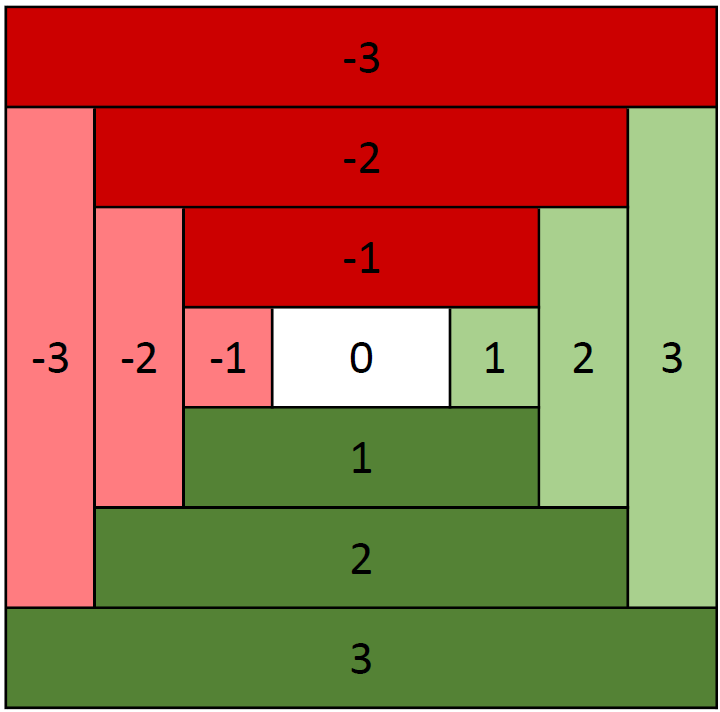
\includegraphics[scale=0.5]{opti_findnextcar}
\end{figure}
Anschließend wird als letzter schritt innerhalb der letzten schleife noch abgeglichen ob sich ein freies Fahrzeug mit den passenden Koordinaten auf der entsprechenden aktuell geprüften position befinden beispielhaft dargestellt für den Bereich $-y,+x = \{-,+\}$. Aus der Tabelle \ref{tab.1} kann in Verbindung mit den  aktuellen Schleifen variablen die aktuell zu prüfende position bestimmt werden, wie in Beispiel Positionsabgleich zusehen. Zudem wird noch sicherheitshalber ein counter erstellt, der einen exit nach 3 Durchläufen ohne Ergebnis ermöglicht.
\begin{lstlisting}
#Bespiel Positions-Abgleich#
...
elif int(car[c][2].split(";")[0]) == -i
and int(car[c][2].split(";")[1]) == j:
	if car[c][3]== "free":#Requirements: F-S11
    	return car[c]
    else:
        c=c-1
       	cancle = cancle+1
\end{lstlisting}
\begin{table}[h]
\centering
\label{tab.1}
\caption{Abgleich-Tabelle für die Positionsbestimmung der fahrzeuge}
\begin{tabular}{lcccccr}
--,--&--,-&--,=&--,+&--,++\\
-,--&-,-&-,=&-,+&-,++\\
=,--&=,-&=,=&=,+&=,++\\
+,--&+,-&+,=&+,+&+,++\\
++,--&++,-&++,=&++,+&++,++\\
\end{tabular}
\end{table}
Als Rückgabewert wird der Datensatz des Fahrzeugs, dass dem Kunden am nächsten liegt an den Aufruf zurück gegeben, dieser kann anschließend an den Kunden übermittelt werden.
\subsection{Ankunft am Ziel}
Für den Server ist durch die Vermittlung des nächstgelegenen Fahrzeugs an den Kunden der Hauptteil seiner Aufgabe erledigt und das Primärziel erreicht. Demnach wurde dem Kunde auf effiziente weise ein Fahrzeug vermittelt und im falle einer Buchung eines Service Fahrzeug im Optimalfall sogar leben gerettet. Allerdings stehen nicht unbegrenzt Fahrzeug Ressourcen zur verfügen, weswegen eine einfach Nutzung dieser im realen Umfeld logischer weise niemals Anwendung finden würde. Des wegen ist es zwingend erforderlich eine Möglichkeit zu bieten Fahrzeuge fortlaufend an Kunden zu vermitteln.\\
Da aufgrund der zu beginn des Projektes beschriebenen Systemumgebung, der Server seinen Einfluss an den  georderten Fahrzeug  mit der Übermittlung der Fahrzeug Daten zum Kunden an  diesen die Kontroll-Gewalt abgibt. \cite[?] ist es dem Server erst durch Initiative des Kunden möglich Fahrzeuge wieder in den Status free zu nehmen. Dieses verfahren bieten auf einen erste logische Betrachtung die Vorteile, dass solange der Kunde nicht aussteigt ein Fahrzeug auf keinen Fall frei werden kann, dies kommt der Praxis sehr nahe und bildet deswegen sehr gut die Realität ab. Ein Nachteil für dieses vorgehen ist allerdings das durch die Abgabe der Kontroll-Gewalt der Server keinen Einfluss mehr auf das Fahrzeug hat, solange es nicht durch die Nachricht des Kunden Freigegeben wird, sollte nun der Kunde aussteigen und   keine Nachricht an den Server senden, oder sollte diese verloren gehen, so wird dieses Fahrzeug auf unbegrenzte zeit als belegt verbucht bleiben und somit nicht genutzt werden können. \\ Eine Lösung des Problems wäre ein timer, der nach einer bestimmten zeit eine anfrage an jedes Belegte Fahrzeug sendet, ob dies immer noch durch den Kunden belegt ist. Des weiteren könnte eine Rückanmeldung eines Fahrzeug auch auf Nachricht des Fahrzeugs umgesetzt werden, so das das Fahrzeug sich in dem Moment des frei Werdens beim Server zurück anmeldet.
Allerdings würde der verwendete Kern code auch in beiden optimierungs fällen ähnliche Funktionen aufweisen.
\\
Eine Nachricht zur freigabe eines Fahrzeugs wird mittels einer Nachricht über den Kanal \textsf{"hshl/mqtt\_exercise/user/"id"/status/reset"} und dem Inhalt "type" , "id" des Users und der id des Fahrzeugs "idCar" an den Server gesendet, dieser ist nun in der Lage durch den Aufruf der Funktion \textit{$statusReset(int(js["idCar"]),str(js["type"]))$} mittels Fahrzeugtyp und dessen ID, dem benutzte Fahrzeug wieder den Status free zu zu ordnen, ein weiterer wichtiger schritt wird mittels Funktionsaufruf
\textit{$requestPosition(js["idCar"],js["type"],\\str(findcarname(js["idCar"],str(js["type"]))))$}
vollzogen.  Angefragt wird der Aktuelle Standort des freigegebenen Fahrzeugs um in fortlaufenden Buchungen wieder die Möglichkeit zu bieten dem Kunden sein nächstgelegenes Fahrzeug zu Verfügung zu stellen. demnach sendet der server dem gerade freigegebenen Fahrzeug über den Kanal \textsf{"hshl/mqtt\_exercise/get\_position"} eine anfrage mit dem Inhalt "id" des Fahrzeugs und dem dazu gehörigen Namen und erhält im besten Fall  eine Antwort über den Kanal  \textsf{"hshl/mqtt\_exercise/set\_position} mit Informationen über "id" des Fahrzeugs,seines "typs" und zuletzt der aktuellen "coordinates". Diese Informationen werden dann in der passenden liste des Typs für das aktuelle Fahrzeug aktualisiert.
\begin{lstlisting}
    data = {
    "type": cartype,
    "id": id,
    "idCar": idCar,
    }
\end{lstlisting}
\subsection{Periodische Abfrage der Fahrzeugposition}
In der Realität stehen Fahrzeuge wie Taxen oder Polizeifahrzeuge selten still. Aus diesem Grund ist die Wahrscheinlichkeit ziemlich hoch, das diese Fahrzeuge nach ihrer Anmeldung im laufe der Zeit ihre Position verändern. Deswegen erscheint es nur sinnvoll in Regelmäßigen abständen dessen position zu kontrollieren beziehungsweise abzufragen, um immer zu garantieren, das das nächst gelegene Fahrzeug ausgewählt werden kann.\\ Problematisch ist hierbei, dass die menge an zu überprüfenden Fahrzeugen einen erheblichen Zeitaufwand in Anspruch nimmt und somit nicht so schnell wie möglich auf anfragen eines Clients reagiert werden kann oder im schlimmsten Fall sogar Nachrichten verloren gehen können. Aufgrund dessen ist es notwendig die Abläufe von Nachrichten Verarbeitung und Abfrage der Position von einander zu trennen. Genutzt wurde hierfür die Möglichkeit, mittels Python Erweiterung \textbf{threading} auf Multi-Threading setze und somit die Aufgaben in 2 verschiedenen Prozessen aufzusplitten. Dies hat zwar zur folge, das die Auslastung des ausführenden system ein wenig höher ist, allerdings sind selbst Einplatinen Computer schon seit längerem mit Mehrkern Prozessoren ausgestattet, was jegliches bedenken bezüglich der Auslastung ihm rahmen dieses Projektes hinfällig macht.
